% !TeX spellcheck = en_US
% !TeX encoding = UTF-8
\chapter{Conclusion}

In this section we will look at some of the limitations and drawback of our approach as well look at future work and research direction that can be taken.

\section{Limitations and Future Work \gls*{gptmo}}


In our research on stress analysis, we primarily relied on subjective measures for labeling and establishing ground truth. While many previous studies have successfully employed this approach, it is important to acknowledge that subjective ratings can be influenced by a variety of factors. These influences could range from individual perception differences to contextual and environmental factors impacting a participant's response. Consequently, reducing the complex and multifaceted nature of stress into a three-class system based on subjective assessments might lead to oversimplifications of the nuanced nature of stress.
Our approach, while aligned with standard practices in stress research, does acknowledge the limitations inherent in using subjective measures for stress categorization.

Since our study only used supervised machine learning to classify the stress level.
For future research, it could be suggested to employ deep learning techniques or a combination of multiple deep learning approaches directly on raw multimodal sensor data, to identify stress levels in human-robot interactions without the need for manual feature crafting. Additionally, unsupervised learning could be explored to autonomously discover features related to stress from unlabeled sensor data. The study's sample size was limited, with a small group of participants and a few levels of stress categorization. Although the sample size followed precedents in related research, it may limit the applicability of the findings in broader human-robot collaboration contexts. Future studies should aim to collect more extensive datasets representing a wider range of stress states to enhance the generalizability of the results to a broader population involved in human-robot collaboration


\begin{figure}[!htbp]
	\centering
	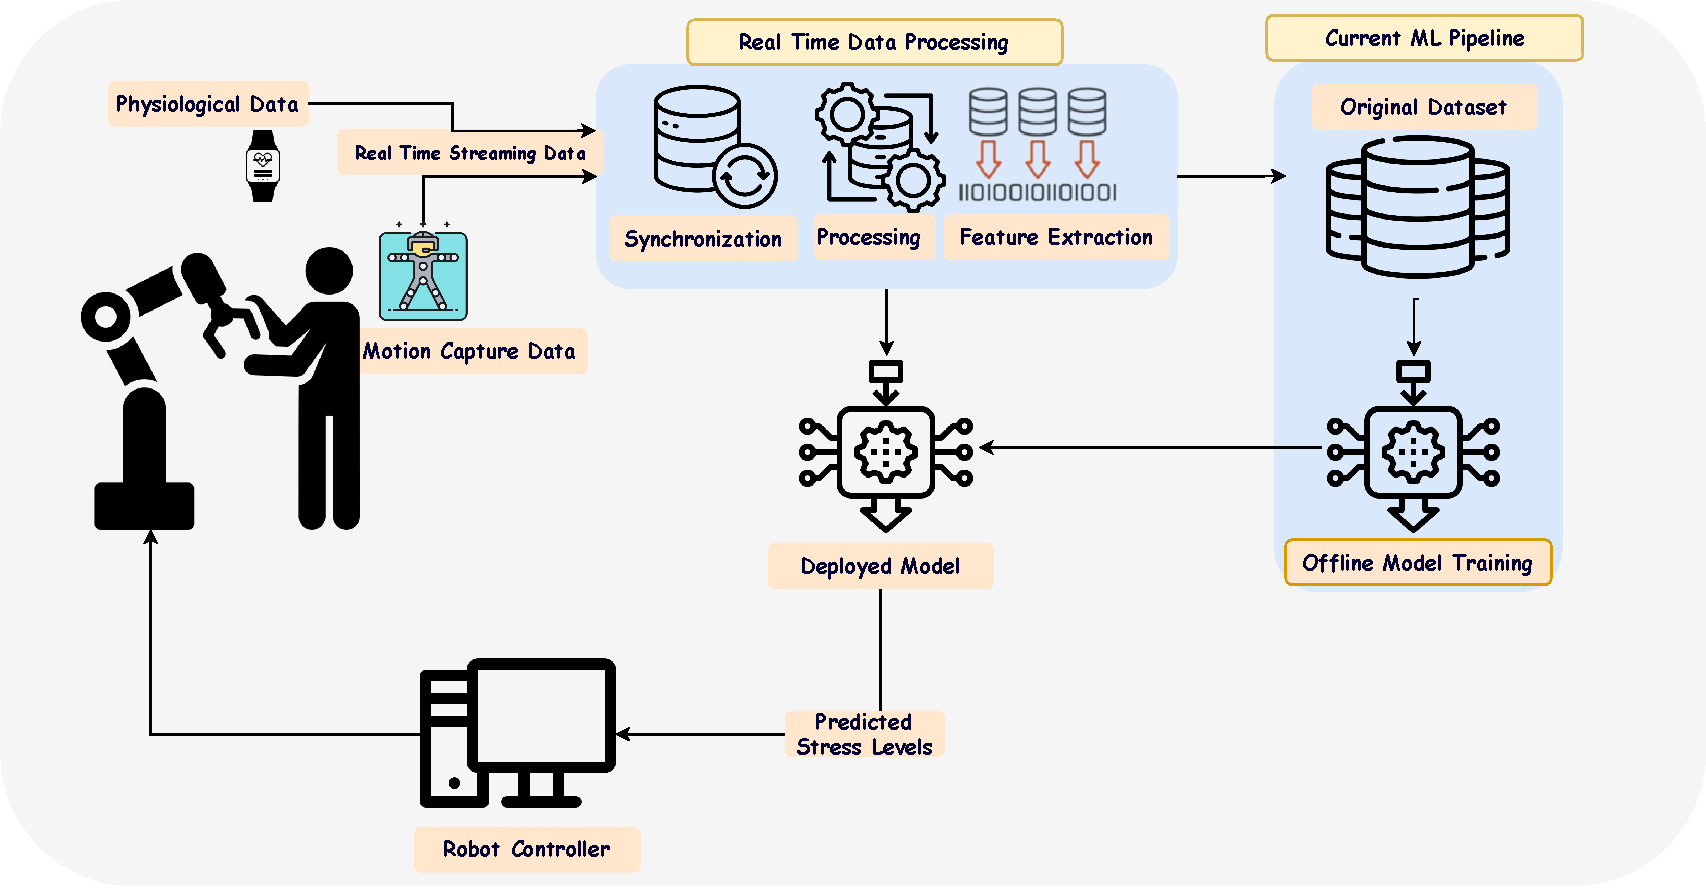
\includegraphics[width=\columnwidth]{images/onlineschematic.drawio (1).pdf}
	\caption{Proposed system with feedback to robot controller based on stress values}
	\label{fig:fut}
\end{figure}


Also, other future work can include a real-time stress monitoring and feedback to the robot controller system.
One of the primary motivations behind our research is to assess human stress levels with the goal of developing a robust machine learning model that can accurately predict stress. This model would serve a pivotal role in real-world applications, particularly in enhancing the quality of human-robot interactions and contributing to the field of affective robotics. By understanding and predicting stress levels, we aim to develop adaptive robot controllers that can respond to the nuanced signals of human operators, thereby managing stress effectively and improving the efficiency and safety of HRI tasks.

A schematic representation of this proposed system is shown in \autoref{fig:fut}. The physiological and motion capture data of the human working in collaboration of a \gls{Cobots} can be streamed in real-time. 
These then undergo various preprocessing steps such as data cleaning, synchronization, and feature extraction which is then fed to our deployed model to predict the current stress levels.
This information can be then fed to the robot's controller, enabling it to adjust its behavior in response to the user's state, slowing or pausing if stress escalates.
This creates a dynamic, responsive environment where the robot's actions are informed by the human's state, enhancing safety and synergy in the human-robot collaboration.

Also in our current setup, we employ a marker-based motion capture system with an array of 12 cameras to accurately track human movement. However, recent advancements in 3D pose estimation technology suggest the feasibility of achieving similar results with simpler setups, such as stereo camera configurations or even single-camera systems\parencite{luvizon2023sceneaware}. These advancements have the potential to reduce the complexity and cost of the system, making it more accessible and scalable for a wide range of applications.


Other suggestions could be as eluded in \autoref{sec:result}, a hybrid approach that utilises Predictive Collision Avoidance for general movement and switches to Dynamic Collision Avoidance for handover situations. By leveraging the strengths of both Dynamic and Predictive Collision Avoidance strategies, we can enhance the interaction experience between humans and robots.A system that uses Predictive Collision Avoidance to navigate general movement paths, where predicting human motion is could feasible and beneficial. However, when it comes to critical interaction points, like handovers, the system could switch to Dynamic Collision Avoidance to allow for real-time adjustments based on actual human movements.


By integrating these elements into a cohesive system, we are working towards robots that are not only more autonomous but also empathetic to the human experience, paving the way for a new era of collaborative workspaces where human well-being is a priority.




\section{Conclusion}

In conclusion, this thesis has made significant strides towards understanding and addressing the complex dynamics of human stress in the context of human-robot interaction. The primary objective was to evaluate the impact of varying collision avoidance strategies on human stress levels, a goal that was approached through a multifaceted study design. This involved a careful analysis of different robot collision avoidance strategies and their interaction with various collaboration levels and robot control strategies.
A holistic approach was developed for evaluating stress levels in human-robot interactions. This involved combining objective physiological measures such as BVP, EDA, HR, and body posture analysis with subjective experiences gathered through participant questionnaires. This dual approach provided a rich and nuanced understanding of stress in human-robot interactions.
A sophisticated system was designed to gather data from multiple sensors operating at different frequencies. This included the use of devices like the Empatica E4 wristband for capturing BVP and EDA, as well as a motion capture system to record human posture and movement. A crucial aspect of this setup was the synchronization of these diverse data streams, ensuring accurate and consistent assessment of human physiological states across different scenarios.
The data obtained from these extensive measurements were then utilised to develop a predictive machine learning model. This model is capable of identifying and addressing sources of stress during human-robot collaboration, thereby contributing to the safer and more effective design of human-robot interaction environments.

The findings from this research provide valuable insights into the relationship between robot collision avoidance strategies and human stress. They underscore the importance of considering human well-being in the design of robotic systems and highlight the potential of machine learning and physiological measurement in enhancing our understanding of human-robot interaction dynamics.

Future research directions suggested by this study include further refinement of the predictive models, exploring real-time stress monitoring systems, and expanding the scope of the research to include a more diverse range of human-robot interaction scenarios. By continuing to focus on the human aspect of these interactions, future work can build on the foundations laid by this thesis to develop more intuitive, efficient, and stress-reducing human-robot collaborative environments.

%\section{Latex distributions and editors}